\documentclass[12pt,a4paper]{scrartcl}
\usepackage[paper=a4paper,left=30mm,right=18mm,top=25mm,bottom=30mm]{geometry}
\usepackage[ngerman]{babel}
\usepackage[utf8]{inputenc}
\usepackage{ngerman}
\usepackage{graphicx}
\usepackage{fancyhdr}
\usepackage{multicol}
\pagestyle{fancy}

\cfoot{}
\rfoot{\thepage}
\lhead{Maik Wöhl}
\chead{Documentation: Taschenrechner}
\rhead{\today}

\begin{document}
\section*{Documentation}

\begin{center}
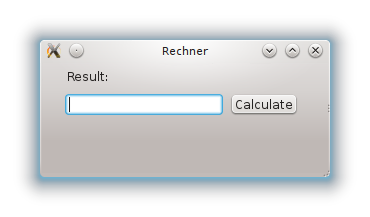
\includegraphics[width=230px,height=130px]{screenshot.png}
\end{center}
This program was developed for the Mono Framework and is ported to Windows Forms. You can choose between many types of mathematical terms that could entered. Behind the GUI works a class that is the same in the CLI-Version. 

Accepted types of mathematical terms are:


\begin{tabular}{|cc|}
\hline
5=5 & Equation Check\\
1+2 & Addition \\
3-2 & Substraction\\
4*3 & Multiplication\\
5/4 & Division\\
6\textasciicircum{}3 & Power\\
sqrt(7) & Square Root\\
sqrt[n](7] & The n-th root\\
lg(8) & 10-logarithm\\
ln(9) & natural logarithm\\
log\_n(10) & logarithm to base n\\
x\textasciicircum{}2 & Parabola\\
-x\textasciicircum{}2 & Negative Parabola\\
-(x-2)\textasciicircum{}2+3 & Shifted Parabola\\
\hline
\end{tabular}
\\
The CLI-Version accepts the following syntax:\\
\texttt{\# mono Taschenrechner1\_CLI.exe Term}\\
or\\
\texttt{\# mono Taschenrecher1\_CLI.exe\\
Enter your term:\\
Term
}
\end{document}